\section{Attention output RMS grows with model depth} 
\label{app:per_tensor_rms_summary}

\begin{figure}[!h]
    % \vspace{4em}
    \centering
    \begin{subfigure}{\textwidth}
        \centering
        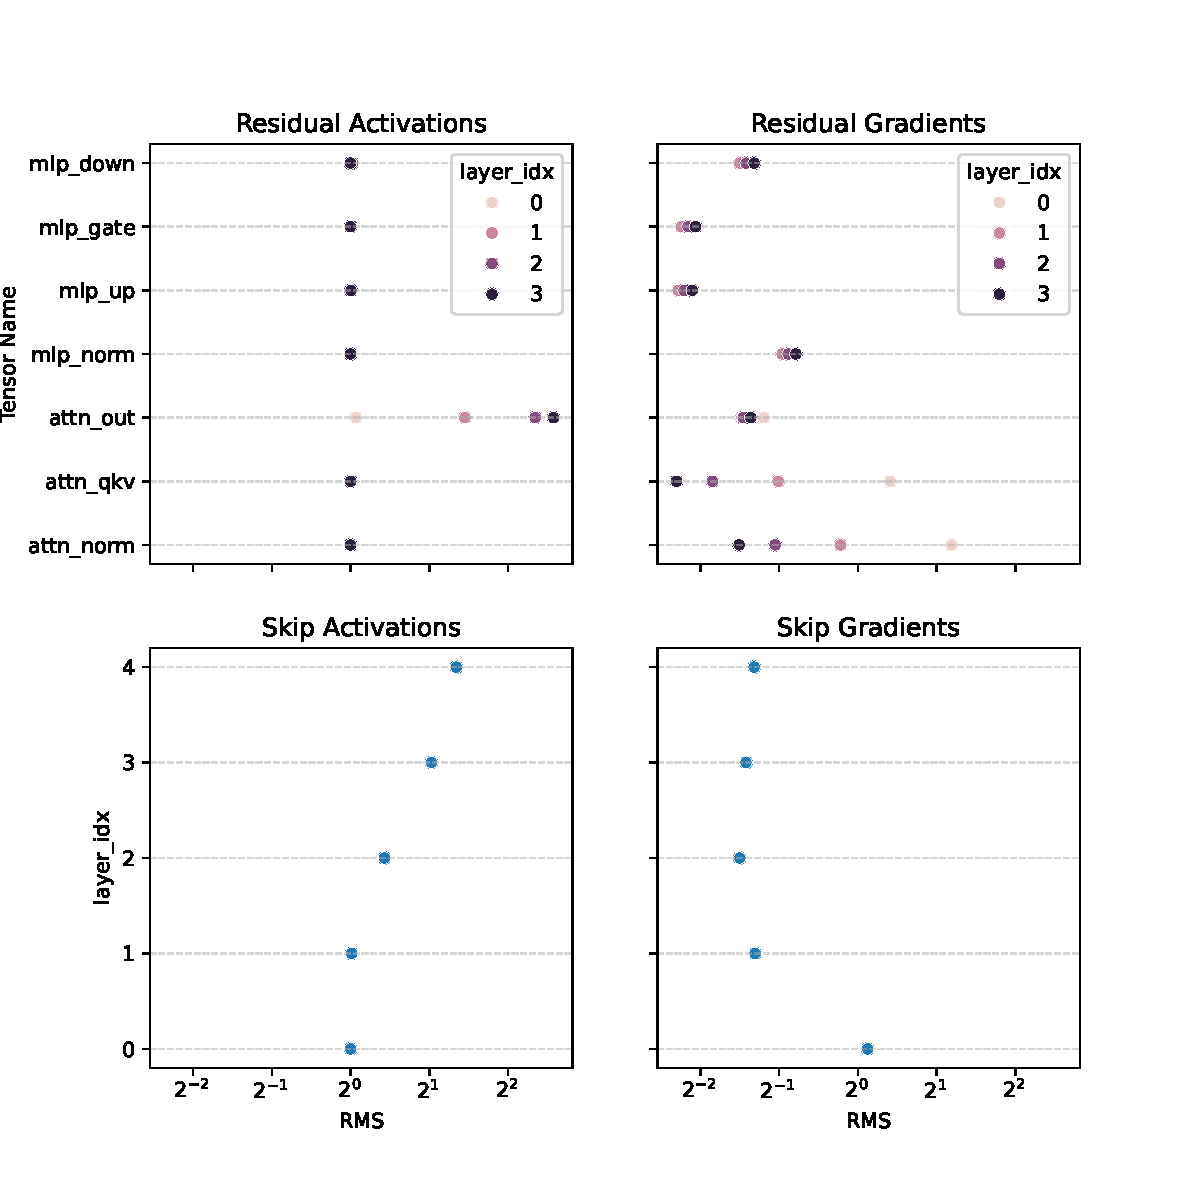
\includegraphics[width=\textwidth]{arXiv/figures/llama-acts-grads-rms.pdf}
    \end{subfigure}
    \caption{Scale of intermediate tensors grows with depth at initialization. Top left: Intermediate activation tensor RMS along the residual branch. Only the attention outputs after the first layer are not unit-scaled. Bottom left: Skip activation tensor RMS. Scale growth in attention outputs drives growth in skip activation scales. Note that \texttt{layer\_idx}$=0$ corresponds to the embedding output, and \texttt{layer\_idx}$=4$ corresponds to the final layer outputs. Top right: Intermediate gradient tensor RMS along the residual branch. Growth in the attention output scale drives growth in attention qkv gradient scales. Bottom Right: Skip gradient tensor RMS. The scale of output activations induces a global rescaling of the gradients.}
    \label{fig:acts-grads-rms}
\end{figure}

A core assumption in deriving per-op scaling factors is that each input to an operation has zero mean, unit-variance, and uncorrelated elements at initialization. This is trivially true for weights and by extension the token embeddings taken as input to the transformer trunk. However, this is not guaranteed for intermediate results and gradients if an operation in the computational graph induces correlation in the elements. In such a scenario our scaling factors will not return unit-variance outputs as we will not have corrected for these correlations in the inputs. As we then increase the depth of the network, where the same operation is left to amplify correlations, we can end up with variance in intermediate results and gradients scaling with depth

Figure \ref{fig:acts-grads-rms} illustrates this phenomenon in a unit-scaled four-layer Llama model with width=256. All activation tensors in the residual branches are unit-scaled, except for the output of the attention layers. We also see that the variance of attention outputs grows with depth. Since Llama models use pre-norm on the residual-branch, residual-branch inputs will revert to unit-scale again until they reach another instance of the correlation-inducing operation. As we add under-scaled attention layer results back to the skip-branch, our skip tensor variances grow with depth as our residual-add assumes unit-variance inputs. This has a knock-on effect on the global scaling of the gradients since the Jacobian of the final norm will scale the gradient by the inverse of the final skip tensor variance.

So which operation induces correlation in the attention output at initialization? For the default case where all multipliers are set to 1, our $1/d$ scaling of attention logits results in a sufficiently high temperature that attention probabilities are effectively uniform. With causal masking, we effectively take a running mean across the value tensor along the sequence dimension. As a result, each subsequent token representation is correlated with the last. Since we derive appropriate scaling factors for the first layer, we do not see scale growth emerging until the second layer, where correlations accumulate during the next effective running mean.

We leave it to future work to offer a solution to scale growth created by correlation in intermediate tensors. We note that this is scale growth emergent at initialization, but we also see scale growth in other intermediate tensors during training. Whether scale growth during training is related to the phenomenon outlined here remains to be seen.